\documentclass{article} % For LaTeX2e
\usepackage{nips15submit_e,times}
\usepackage{hyperref}
\usepackage{url}
\usepackage{graphicx}
%\documentstyle[nips14submit_09,times,art10]{article} % For LaTeX 2.09


\title{GuineaPig Naive Bayes for 10605 15 Fall}


\author{
Jingyuan Liu\\
AndrewId: jingyual\\
\texttt{jingyual@andrew.cmu.edu} \\
}


\newcommand{\fix}{\marginpar{FIX}}
\newcommand{\new}{\marginpar{NEW}}


\nipsfinalcopy % Uncomment for camera-ready version


\begin{document}
\maketitle


\section{Question 1}


I did not recieve direct help from others. I did not give detailed direct help to others.


\section{Question 2}
We could use following steps to generate the required output:

\textbf{Step 1}, Group all the files to get the fg count. Using GunieaPig
like represenatation:

\qquad fgCount=Group(by=lambda (n,y,c):y=1960,reducingTo=ReduceToCount)

\textbf{Step2}, Group all the files to get the bg count. Using GunieaPig like
represenatation:

\qquad bgCount=Group(by=lambda (n,y,c):y$>$1960,reductingTo=ReduceTocount)

\textbf{Step3}, After getting the two tables, we could join the two tables by the word
names and then map it to the format we want:

\qquad joined=Join(Jin(fgCount, by=lambda (n,y,c):n), Jin(bgCount,
by=lambda (n,y,c):n))

\qquad output= Map(joined, by=formatting)

After these three steps, we could get the formatted output as required.

\section{Question 3}

\subsection{(a)}
The figure is as follows, the runtime is measured in seconds.
\begin{figure}[h]
\begin{center}
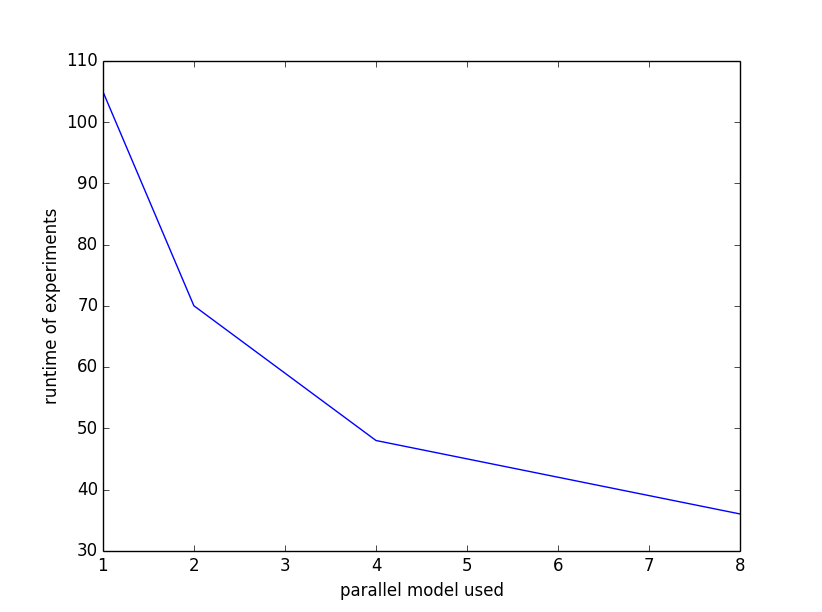
\includegraphics[width=8cm]{pic/run.png}
\end{center}
\caption{runtime vs. parallel models}
\label{fig:monitoring}
\end{figure}


\subsection{(b)}
As we could see from the figure above, the program is not perfectly scalable.
The running time would not halves if the number of worker machine is doubled.
This was due to several reasons. First of all, sperating data to different
machines would cost extra running time compared with running on a single
machine. Besides, when it comes to distributed computing paradigm, the
synchronization would always take extra time. When we need do the whole corpus
reducing, faster machines would need to wait for slow machines to finish their
mapping or combining job, then started reducing jobs.

For my program, in the mapping step, I scanned twice the whole corpus to get all
the parameters and counts. The faster machines would wait for the slower
machines in these two scans for next actions. Then the join step, it would cost
extra time to distribute data to different machines


\section{Question 4}
This is a quiet interesting problem. We should treat the two tables as streams
in order to process the dataset in limited memory. So just like we are
processing data between Map and Reduce steps in Hadoop, we need to sort the
data, and then read the data stream. In order to get the distinct products, we
could also sort the productId, or we could use a set to store distinct value.
To get the counts, we need previous keys to store the past value and compare
with current value.

\textbf{Step 1}. Sort two tables. The time complexity is $o(n_1 logn_1+n_2logn_2)$ $n_1,
n_2$ is table size. We could also only sort one table, and then stream another
table and binary search the key in the sorted table. This would cost
$(n_1logn_1)$.

\textbf{Step 2}. Loop sorted tables. Then we could read the stream data from the two
sorted tables. We first read id1 from table1 and get name. Then we read id2
from table2. If the id1 == id2, go to Step 3. If id1 $<$ id2, id1++. If id1
$>$ id2, id2++. Loop the two sorted table would be $o(n_1+n_2)$. If we only
sorted one data, and use binary search here, then the time would be
$o(n_2logn_1)$

\textbf{Step 3}. Get distinct products count. If id1 matches id2, then we could get the
distinct products that person bought. We could first sort and then loop the
productIds. If the previousKey does not eauql currentKey, then add one to the
count. This would cost $o(mlogm + m)$ for time, and o(1) for space. We could
also use a set to store different productIds. This would cost $o(m)$ for time,
but o(m) for space.

With these three steps, we could implement the Join and Distinct functions in
GuineaPig, getting name and distinct count. The time complexity is about
o(nlogn + n) and with limit space complexity, which are aceeptable.


\section{Question 5}
The meaning of each python code line is :


\textbf{L1} doc = ReadLines('data.txt') | Map(by=lambda line:line.split(" "))

\qquad This line would read data and then split each line via space into a list.

\textbf{L2} t1 = Flatten(doc, flat1)

\qquad This line get the even index word from the splited doc

\textbf{L3} t2 = Flatten(doc, flat2)

\qquad This line get the odd index word from the splited doc

\textbf{L4} t3 = Join(Jin(t1), Jin(t2)) $\mid$ ReplaceEach(by=lambda(w1,w2):(w1+w2,len(W2)))

\qquad This line would first join the two views, and get a word tuple. The first
element is the even index word, and the second element is the nearest bigger odd
index word. In the joined result, the w1 = w2. Then it would map the joined table
to a new tuple. The new first elment is the word1 + word2, the new second element
is the length of word2.


\end{document}
